\cleardoublepage

\chapter{Rozpoznanie dużych modeli językowych}
W niniejszym rozdziale autor przybliżył dziedziny, w których generatywna sztuczna inteligencja może wspomagać ludzką kreatywność, zapewniając przy tym oszczędność czasu. Dodatkowo, opisał skomplikowaną architekturę transformer, która stanowi podstawę działania dużych modeli językowych. One także zostały dokładnie i praktycznie opisane w ostatnim podrozdziale.


    \section{Generatywna sztuczna inteligencja}
    Termin \enquote{generatywna sztuczna inteligencja} (ang. \textit{generative artificial intelligence} — GenAI) nie schodzi z ust ludzi na całym świecie od 30 listopada 2022. Tego dnia opublikowano chatbota ChatGPT, który zrewolucjonizował formę kreatywnej komunikacji człowiek-komputer. Modele generatywne nie tylko zaczęły tworzyć tekst na zaawansowanym poziomie, ale także obrazy, muzykę, filmy czy oprogramowanie. Jak słusznie opisano w książce \cite{genAI_langchain2024} \enquote{te modele mogą zapewnić bardzo wiele funkcjonalności, między innymi wyszukiwanie semantyczne, manipulowanie zawartością oraz klasyfikację}. Dzięki tym rozwiązaniom, wykorzystując automatyzację, łatwo zredukowano koszty, a ludzka kreatywność wzrosła do niespotykanego dotąd stopnia.
        

        \subsection{Generowanie tekstu}
        Jednym z najczęstszych zastosowań GenAI jest tworzenie nowych treści w języku naturalnym. Modele takie jak GPT-4, opracowany przez amerykańską firmę OpenAI, mogą być wykorzystywane do streszczania długich treści, pisania artykułów czy rozwiązywania równań matematycznych z pełnym opisem toku rozumowania. Wytrenowane na ogromnych zbiorach tekstu, posługują się średnio ponad osiemdziesięcioma językami, co czyni je perfekcyjnymi tłumaczami.
        
        
        \subsection{Generowanie obrazu}
        W 2014 roku Ian Goodfellow zdefiniował architekturę sieci Generative Adversarial Network (GAN) służącej do generowania realistycznych obrazów. W praktyce niemal niemożliwe jest odróżnienie obrazu wygenerowanego od rzeczywistego. W 2021 roku firma OpenAI wdrożyła DALL-E — nowy i innowacyjny generatywny model. W przeciwieństwie do poprzedniej architektury, ta umożliwiła tworzenie obrazów na podstawie tekstu w języku naturalnym (ang. \textit{text-to-image}). Generowanie obrazu umożliwia poszerzanie zbiorów treningowych (augmentację danych) dla wizji komputerowej, tworzenie bardziej kreatywnych grafik w marketingu czy projektowanie nowych produktów cyfrowych.
        
        
        \subsection{Generowanie muzyki}
        Illiac Suite jest pierwszym utworem muzycznym w pełni skomponowanym przez sztuczną inteligencję. Jego pomysłodawcami byli Lejaren Hiller i Leaonardo Isaacson w 1957 roku. Od tamtej pory bez przerwy rozwijano techniki generowania muzyki. W 2016 roku firma Google zaprezentowała otwartoźródłowy projekt badawczy Magenta. Wykorzystano w nim głównie rekurencyjne sieci neuronowe. Cztery lata później OpenAI zaprezentowało Jukebox \cite{dhariwal2020jukebox}. Jest to sieć neuronowa generująca muzykę, dzięki której użytkownik posiada kontrolę nad gatunkiem, głosem artysty oraz stylem muzycznym utworu.

        
        \subsection{Generowanie wideo}
        Rozwój powyższych trzech dziedzin generowania treści w ostatnich latach przyczynił się do zaawansowanego rozwoju generowania wideo. Na dzień dzisiejszy, do najpopularniejszych rozwiązań zalicza się Runway Gen-4.5, OpenAI Sora oraz Google Veo. Każde z nich umożliwia tworzenie realistycznych lub stylizowanych materiałów wideo na podstawie obrazów lub zapytania tekstowego. Przytoczone oprogramowania najlepiej radzą sobie przy tworzeniu krótkich, kilkuminutowych treści. Z jednej strony technologia ta otwiera szereg nowych możliwości w pracy artystów czy twórców internetowych. Z drugiej zaś strony, za pomocą fałszywych treści wideo (ang. \textit{deepfake}) coraz częściej dochodzi do manipulacji społeczeństwa na platformach społecznościowych i w mediach.

        
        \subsection{Wpływ na środowisko}
        W celu obsługi i rozwijania modeli generatywnych na szeroką skalę, wymagana jest ogromna moc obliczeniowa. Wytrenowanie pojedynczego modelu potrafi zużyć nawet 50 GWh energii. Dzieje się tak, ponieważ wymagane jest do tego wykorzystanie tysięcy procesorów graficznych (ang. \textit{graphics processing unit} — GPU), wykonujących obliczenia przez wiele tygodni. Utrzymanie infrastruktury, w tym odpowiadanie na zapytania (prompty), kiedy model generatywny jest wdrożony na rynek, także kosztuje olbrzymią ilość energii każdego dnia.

        
        \subsection{Prawa autorskie}
        Relacja między GenAI a prawem jest wciąż dynamicznie kształtowana. Obecnie, zgodnie z obowiązującym prawem w Polsce i UE, tylko człowiek może być autorem wszelkich treści kreatywnych. Jeżeli coś zostało automatycznie wygenerowane przez sztuczną inteligencję, bez zasadniczego wkładu intelektualnego człowieka, nie podlega to ochronie praw autorskich.

        
        \subsection{Ogólna sztuczna inteligencja}
        Ogólna sztuczna inteligencja (ang. \textit{artificial general intelligence} — AGI) jest koncepcją rozwoju sztucznej inteligencji do poziomu ogólnej adaptacji i zdolności do absorbowania wiedzy z różnych dziedzin. W swoim zamyśle, AGI osiągnie poziom inteligencji zbliżony do ludzkiego. Jak trafnie opisał autor artykułu \cite{agi2014}, system wykazujący się ogólną sztuczną inteligencją powinien generalizować wiedzę, co umożliwi jej transferowanie między różnymi problemami i kontekstami.

        
    \section{Architektura transformer}
    Problemem tradycyjnych modeli takich jak RNN, LSTM czy GRU, przetwarzających dane sekwencyjnie, jest gubienie kontekstu dłuższych treści. Reprezentacja każdego tokena zależy od poprzednich tokenów z ciągu oraz od niego samego, ograniczając szybkość i wydajność rozwiązania. Jednakże, w 2017 roku firma Google zaprezentowała artykuł \enquote{Attention is all you need} \cite{attention_is_all_you_need2017}, w którym przedstawiono architekturę transformer. Rozwiązanie to nie wykorzystuje złożonych konwolucyjnych czy rekurencyjnych sieci neuronowych, znosząc konieczność przetwarzania sekwencyjnego. Transformer bazuje na mechanizmie samouwagi, inaczej zwanym atencją ze skalowalnym iloczynem skalarnym. Umożliwia to równoległe przetwarzanie danych, wychwytując relacje między bardzo odległymi elementami w sekwencji. Pełny schemat architektury przedstawiono na rysunku \ref{transformer}.

    \begin{center}
        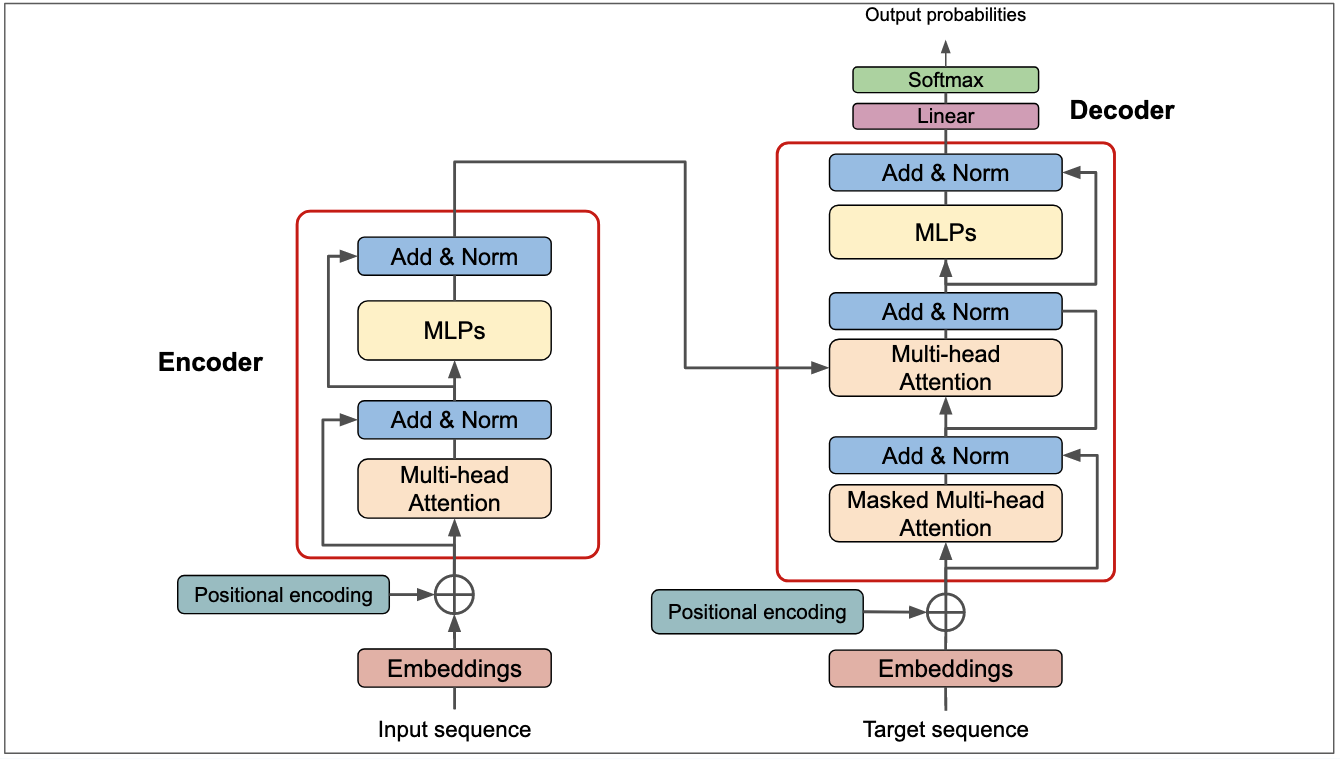
\includegraphics[width=0.75\textwidth]{rysunki/transformer.png}
        \captionof{figure}{ Architektura transformera \cite{attention_is_all_you_need2017}} 
        \label{transformer}
    \end{center}


        \subsection{Tokenizacja}
        Tokenizacja oznacza zamianę tekstu (słów, podwyrazów lub znaków) na wartości liczbowe (tokeny), które są zrozumiałe dla modelu. Jest to pierwszy i najbardziej kluczowy krok, ponieważ sieci neuronowe operują wyłącznie na liczbach i w nich kryje się znaczenie poszczególnych tokenów. Poniżej przedstawiono przykład konwersji tekstu na tokeny wraz z ich numerycznymi identyfikatorami \ref{llm_tokenizer}.

        \begin{center}
            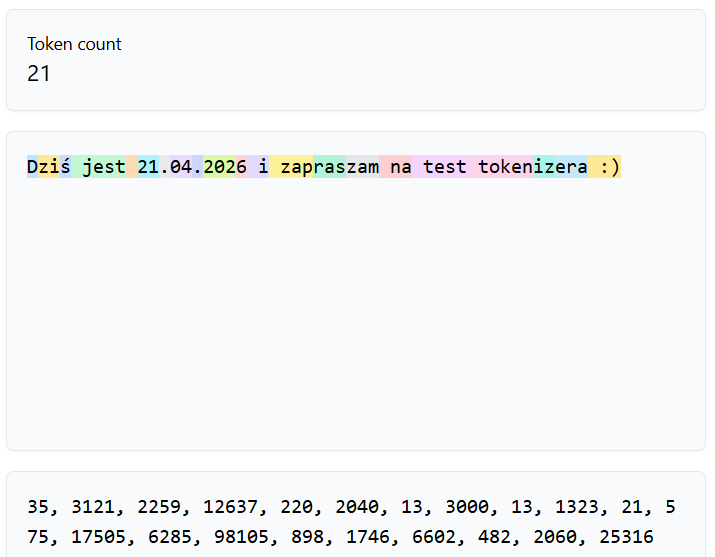
\includegraphics[width=0.5\textwidth]{rysunki/llm_tokenizer.png}
            \captionof{figure}{ Przykład tokenizacji tekstu \cite{tiktokenizer}} 
            \label{llm_tokenizer}
        \end{center}


        \subsection{Reprezentacja wektorowa}
        W następnym kroku, numeryczne identyfikatory tokenów, które są liczbami całkowitymi, przekształcane są w wielowymiarowe wektory liczb rzeczywistych. Tak reprezentowane słowa umiejscowione są w przestrzeni wielowymiarowej, gdzie odległość między wektorami odwzorowuje podobieństwo semantyczne między słowami – im bardziej podobne znaczenia wyrazów, tym bliżej siebie się znajdują. Tę operację nazywa się osadzeniem (ang. \textit{embedding}).
        
        
        \subsection{Kodowanie pozycyjne}
        W transformerze nie ma domyślnie wbudowanej funkcjonalności rozpoznawania kolejności przetwarzanych słów. Odpowiedź na ten problem stanowi kodowanie pozycyjne (ang. \textit{positional encoding}). Jest to technika, która umożliwia podanie do transformera informacji dotyczącej pozycji tokenów w sekwencji. Polega na tym, że do każdego wektora embeddingu dodawany jest wektor jego pozycji.
        
        
        \subsection{Mechanizm samouwagi}
        Mechanizm samouwagi (ang. \textit{self-attention mechanism}) umożliwia modelowi analizowanie różnych fragmentów na raz, zamiast przetwarzać dane wejściowe w kolejności. Algorytm wylicza wagi uwagi określające względną ważność każdej części tekstu w sekwencji. Następnie stosuje te wagi, aby zmniejszyć lub zwiększyć wpływ analizowanych fragmentów na predykcję transformera.

        
        \subsection{Koder i dekoder}
        Zadaniem kodera (ang. \textit{encoder}) jest pobranie sekwencji danych na wejściu i generowanie sekwencji stanów ukrytych, z których każdy jest sumą ważoną wszystkich operacji osadzenia (embeddingu) danych wejściowych. Z kolei dekoder (ang. \textit{decoder}), otrzymując sekwencję danych wyjściowych, przesuniętą w prawo o jedną pozycję, generuje sekwencję estymacji. Każda z nich jest sumą ważoną stanów ukrytych kodera, zależną od poprzedniego stanu dekodera \cite{llm_w_proj_oprogramowania2024}. Na końcu dekodera dochodzi do konwersji surowych wartości mechanizmu uwagi (tzw. logitów) na rozkład prawdopodobieństwa możliwych odpowiedzi (tokenów). Odbywa się to za pomocą funkcji softmax.
        
    
    \section{Definicja dużego modelu językowego}
    Dużym modelem językowym (ang. \textit{large language model} — LLM) nazywamy algorytm oparty na uczeniu głębokim, który posiada miliardy wewnętrznych parametrów (wag) i został wytrenowany na gigantycznych zbiorach danych. Zbudowany jest na podstawie zdefiniowanej wyżej architektury transformer. Model stworzony został do wykonywania wielu zadań związanych z przetwarzaniem języka naturalnego, takich jak generowanie, tłumaczenie czy podsumowywanie tekstu \cite{llm_w_proj_oprogramowania2024}. Warto podkreślić, iż duże modele językowe nie \enquote{myślą} w sensie ludzkim, lecz estymują kolejny najbardziej prawdopodobny token w oparciu o tekst na wejściu. Są one dostępne dla szerokiego grona odbiorców dzięki dedykowanym interfejsom użytkownika (chatbotom) oraz API. Specyfikę najpopularniejszych z nich przybliżono w poniższym podrozdziale.

    
        \subsection{Przegląd popularnych dużych modeli językowych}
        Pierwszym rozpatrywanym dużym modelem językowym jest Generative Pre-trained Transformer (GPT). Został stworzony przez założoną w 2015 roku amerykańską firmę OpenAI, która obecnie jest liderem w dziedzinie generatywnej sztucznej inteligencji. Model GPT jest wstępnie wytrenowany (ang. \textit{pre-trained}) na ogromnych zbiorach nieetykietowanych danych, dzięki czemu nabywa ogólne zdolności językowe i staje się wszechstronną bazą, która posiada możliwość dostrojenia do konkretnych zadań. Pierwszym produktem firmy, wykorzystującym architekturę transformer, był GPT-1 stworzony w 2018 roku. Sukces rodziny modeli GPT, szczególnie od 2022 roku za sprawą wydania aplikacji ChatGPT bazującej na modelu GPT-3.5, stał się katalizatorem, który zmusił konkurencję do zintensyfikowania prac nad własnymi rozwiązaniami AI. Nowsze modele, na przykład GPT-4o, nie tylko przetwarzają tekst, ale także dźwięk i obraz.

        Założona w 2023 roku chińska firma Hangzhou DeepSeek Artificial Intelligence Basic Technology Research w 2025 roku wdrożyła na rynek porównywalnego chatbota DeepSeek. Wykorzystywał znacznie tańszy otwartoźródłowy model DeepSeek-R1 o osiągach porównywalnych do GPT-4, co stanowiło ogromną konkurencję dla produktów firmy OpenAI. Co więcej, chińske przedsiębiorstwo przyznało, że trening ich modelu był kilkanaście razy tańszy i zużywał do dziesięciu razy mniej mocy obliczeniowej niż konkurencyjne modele. Poza podstawową architekturą transformer, modele DeepSeek wykorzystują dwa dodatkowe podejścia w celu poprawy ich wydajności — strategię trenowania modelu wolną od strat pomocniczych (ang. \textit{auxiliary-loss-free strategy}) oraz strategię celu treningowego polegającego na przewidywaniu wielu tokenów jednocześnie \cite{deepseek_technical_report2024}.

        Trzecim prezentowanym modelem jest Gemini od amerykańskiej firmy Google, wcześniej znanym pod nazwą Bard. Jako pierwszy, w 2023 roku, zadebiutował wariant Gemini 1.0. Rodzina modeli od Google także bazuje na architekturze transformer. Natomiast, spośród reszty dostępnych modeli, w momencie publikacji Gemini wyróżnił się multimodalnością. Został natywnie zaprojektowany do przetwarzania tekstu, audio, obrazu i wideo na jednym strumieniu danych.

        Claude 1, czyli pierwszy model amerykańskiego przedsiębiorstwa Anthropic, także miał swoją premierę w 2023 roku. Na ten moment, modele rodziny Claude można podzielić na trzy kategorie od najmniej do najbardziej zaawansowanej: Haiku, Sonnet i Opus. Są one najlepszymi modelami na rynku w kontekście analizy i generowania kodu. Modele Claude są trenowane w ramach strategii Constitutional AI, polegającej na dostosowaniu systemów sztucznej inteligencji do ludzkich wartości, czyniąc je pomocnymi, nieszkodliwymi i szczerymi \cite{constitutional_ai2022}.
        
        Ostatnim wartym uwagi modelem jest Grok, stworzony przez amerykańską firmę xAI. Pierwszym ich produktem był Grok-1, wydany w 2023 roku. Poprzez integrację z platformą X, Grok ma aktualną wiedzę dotyczącą bieżących informacji ze świata i trendów. W momencie gdy inne modele dążą do bycia neutralnymi i uprzejmymi w swoich wypowiedziach, Grok jest mniej ocenzurowany, co wpływa na jego skłonności do sarkazmu i bycia bezpośrednim. Jest skłonny do generowania kontrowersyjnych wypowiedzi dotyczących historii, teorii spiskowych, polityki oraz sfery seksualnej.


        \subsection{Ograniczenia modeli LLM}
        Chociaż duże modele językowe są niezwykle popularne i często zaskakująco trafne w swoich wypowiedziach, mają one ograniczenia i niedoskonałości. Poniżej opisano czynniki wpływające na to, że LLMy nie są nieomylne i zawsze jako użytkownicy powinniśmy weryfikować ich wypowiedzi. Warto rozumieć te ograniczenia, aby móc świadomie i skutecznie tworzyć aplikacje bazujące na modelach językowych. Problemy te dowodzą, że ludzka inteligencja i twórczość są niezastąpione.

        Pierwszym czynnikiem ograniczającym skuteczność wypowiedzi w wielu modelach językowych jest nieaktualny stan wiedzy. Jak trafnie opisano w książce \cite{genAI_langchain2024}, \enquote{modele LLM polegają jedynie na danych treningowych, bez integracji z zewnętrznym źródłem danych nie mogą dostarczać aktualnych informacji ze świata}.

        Drugim istotnym powodem, który powinien wzbudzać ograniczone zaufanie jest niedeterministyczne zachowanie. LLMy mogą generować różne, a czasem nawet sprzeczne odpowiedzi na to samo zapytanie (prompt). Wynika to z ich probabilistycznej natury — wyniki zależą od rozkładu prawdopodobieństwa, a nie od sztywno zdefiniowanych reguł. Modele potrafią generować nieprawidłowe lub bezsensowne informacje, ponieważ polegają na wyuczonych wzorcach, a nie na dokładności faktów. Takie zjawisko nazywa się halucynacją.
        
        Kolejnym ważnym aspektem są tendencje modeli do pewnych zachowań czy stronniczości ideologicznych wynikające z danych treningowych. LLMy mogą mieć podłoże religijne, być z natury upolitycznione lub generować treści o charakterze dyskryminacyjnym. Ponadto, przez brak weryfikacji, zbiory danych mogą zawierać fałszywe informacje i szkodliwe porady, które model traktuje jako wzorce do naśladowania.
        
        Inną trudnością jest przyjmowanie właściwego kontekstu przez LLMy. Użytkownik często zakłada, że model \enquote{domyśli się} kim jest, jakie są jego prawdziwe intencje oraz jakie jest tło opisywanej sytuacji. W rzeczywistości, poza promptem, model nie ma innego punktu odniesienia, aby zapewnić nam precyzyjną i rzetelną odpowiedź w złożonych okolicznościach. Dodatkowo, modele językowe mają tendencję do zapominania kontekstu. Mogą one nie pamiętać podanych wcześniej szczegółów w bieżącej czy innej konwersacji.


        \subsection{Dostrajanie modelu}
        Dostrajanie (ang. \textit{fine-tuning}) przeprowadza się na wcześniej wytrenowanym dużym modelu językowym. Ten proces polega na dodatkowym treningu algorytmu na znacznie mniejszym, specyficznym zbiorze danych. Działanie to ma na celu poszerzenie wewnętrznego stanu wiedzy i udoskonalenie modelu do wykonywania dedykowanych zadań \cite{fine_tuning2024}.